\section{Complex and Biologically-Inspired Systems}

\blockquote[Douglas Adams in \textit{The Salmon of Doubt} \cite{adams2002salmon}]{
If you try and take a cat apart to see how it works, the first thing you have on your hands is a nonworking cat.
}

\begin{figure}
\centering
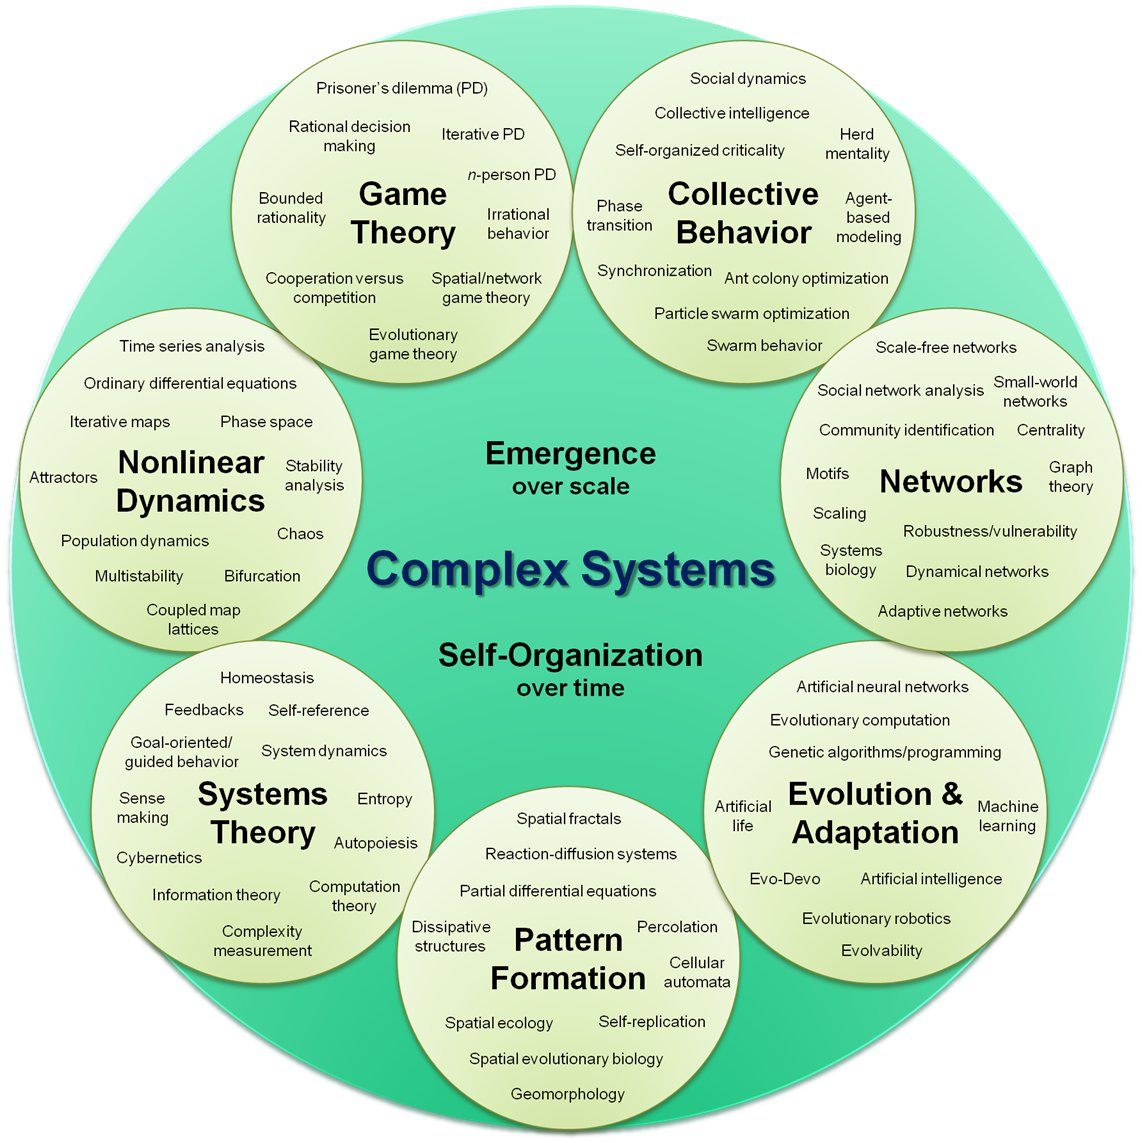
\includegraphics[width=\textwidth]{fig/complex_systems_sayama}
\caption[Complex systems taxonomy]{Complex systems taxonomy. Reproduced from \cite{sayama2015introduction} by Hiroki Sayama.}
\label{fig:complex_systems_taxonomy}
\end{figure}

\textit{Complex systems} is an umbrella category consisting of a variety of topics from a variety of domains, such as mathemathics, computer science and biology.
Figure \ref{fig:complex_systems_taxonomy} shows one possible "taxonomy" of complex systems.
It is not immediately obvious why these topics should be grouped together.
The word \textit{complex} is related to \textit{complicated}, synonymous with \textit{difficult}, \textit{intricate} and \textit{perplexing} \cite{Thesaurus.com2017}.
In 1962, Herbert Simon proposed a definition as \textquote[\cite{simon1962architecture}]{made up of a large number of parts that interact in a nonsimple way}.
Hiroki Sayama later elaborated this as follows:
\blockquote[\cite{sayama2015introduction}]{
Complex systems are networks made of a number of components that interact with each other, typically in a nonlinear fashion.
Complex systems may arise and evolve through self-organization, such that they are neither completely regular nor completely random, permitting the development of emergent behavior at macroscopic scales.
}
Grouping these topics together, it is possible to start seeing similarities across domains, and find insights about one topic that may be applicable to other topics.

A common property of complex systems is \textit{emergence} over scale.
Sayama defines emergence as \textquote{a nontrivial relationship between the properties of a system at microscopic and macroscopic level}.
This means that a process which can be observed at the macroscopic level (e.g. the human body moving) can not be explained by studying the individual components that make up the system (looking at the cells that make up the body).
Instead, both the individual components and \textit{how they interact} must be understood.

The other common property of complex systems is \textit{self-organization} over time.
Sayama defines it as \textquote{a dynamical process by which a system spontaneously forms nontrivial macroscopic structures and/or behaviors over time}.
One example is magnetization of metals, where the initially random configuration of "spins" (the components of the larger system) orient themselves over time,
so that the magnetic vector of all the individual spins and that of the whole system become the same \cite{heylighen2001science}.

The behavior seen in complex systems can be characterized by these two properties.
Often the behavior is a combination of the two properties, rather than a clear instance of one or the other.

Many of the topics seen in Figure \ref{fig:complex_systems_taxonomy} are based on concepts found in nature.
These belong to the group of \textit{bio-inspired systems}.
Since the infancy of modern computing in the 1940s, computers have gradually gained the capability to perform many tasks.
Along the way, computer scientists and engineers have sometimes looked to nature for goals to reach for.
Many times approaching problems from engineering, mathemathical and logical perspectives have yielded good results.
But some times, the analytical approach leads to a dead end.
Some tasks that are trivial for a human to perform, can be practically impossible for a programmer to codify.
This is where the bio-inspired approach may help.
If nature can create biological "machines" that can solve these tasks, then perhaps borrowing nature's methods will allow computers to do the same.
This also gives rise to the field of \textit{artifical life}.

%TODO mention \url{https://en.wikipedia.org/wiki/Moravec\%27s_paradox} ?
